\documentclass[10pt]{article}
\usepackage{amssymb,amsmath,times,url,graphicx,amsthm,alltt}
%\usepackage[pdftex,urlcolor=blue,pdfpagemode=none,pdfstartview=FitH]{hyperref}
\usepackage{my_packages}
\usepackage{tikz_packages}
\usepackage{wasysym}
%% url smaller font.
\makeatletter
\def\url@leostyle{%
  \@ifundefined{selectfont}{\def\UrlFont{\sf}}{\def\UrlFont{\small\ttfamily}}}
\makeatother
\urlstyle{leo}

%\usepackage[all,import]{xy}

\renewcommand{\baselinestretch}{1.2}
\date{}

\renewcommand{\thesubsection}{\arabic{subsection}. }
\renewcommand{\thesubsubsection}{\arabic{subsection}.\arabic{subsubsection} }

\theoremstyle{definition}
\newtheorem{prob}{Problem}[section]
%\renewcommand{\theprob}{\arabic{section}.\arabic{prob}}
\renewcommand{\theprob}{\arabic{prob}}

\newenvironment{subprob}%
{\renewcommand{\theenumi}{\alph{enumi}}\renewcommand{\labelenumi}{(\theenumi)}\begin{enumerate}}%
{\end{enumerate}}%

\newenvironment{matlab}
{\begin{alltt}\small\renewcommand{\baselinestretch}{1.2}\selectfont}%
{\end{alltt}}


\begin{document}



\setcounter{page}{1}
\pagestyle{plain}
\section*{MAE3145: Homework 5}
\vspace*{-0.4cm}
\noindent{Due date: \SI{2458085.2395}{\julianday} }%\\%\vspace*{0.5cm}

\begin{prob}
    Neptune is now the furthest ``planet'' in our solar system (since Pluto is classified as a dwarf planet).
    Voyager 2 passed by Neptune in 1989 but there have not been other spacecraft missions to Neptune.
    Consider a Neptune mission by doing a few preliminary calculations. 

    \begin{subprob}
        \item Begin by examining a Hohmann transfer from the Earth to Neptune.
        Assume that planetary orbits are coplanar and circular.
        Compute the total \( \norm{\Delta \vec v_T} \) and the TOF (time of flight in years).
        Ensure you draw proper vector diagrams, and compute \( \norm{\Delta \vec v}\) and \( \alpha \) for each maneuver.
    \item What is \( \norm{\Delta \vec v_1} \), i.e. the maneuver necessary at Earth departure?
        What is \( \norm{\Delta \vec v_2}\) to remain in the Neptune system?
    \item Discuss the feasibility of this mission.
        Is the total cost (\( \norm{\Delta \vec v_T}\)) ``a lot''?
        Is the time of flight reasonable?
        Even though the Hohmann transfer is the minimum two-impulse transfer, is it likely that we could use this transfer to get to Neptune?
    \item Compare the time of flight you calculated to the actual Voyager 2 transfer. 
        You can use the Julian date functions, \texttt{time.date2jd(yr, mo, day, hr, min, sec)}.
    \item Compute the phase angle required at departure for this circle-to-cirle transfer as seen in the heliocentric view.
    \end{subprob}

    \begin{figure}[htbp]
        \centering
        \subcaptionbox{Voyager 2 Image of Neptune\label{fig:neptune}}{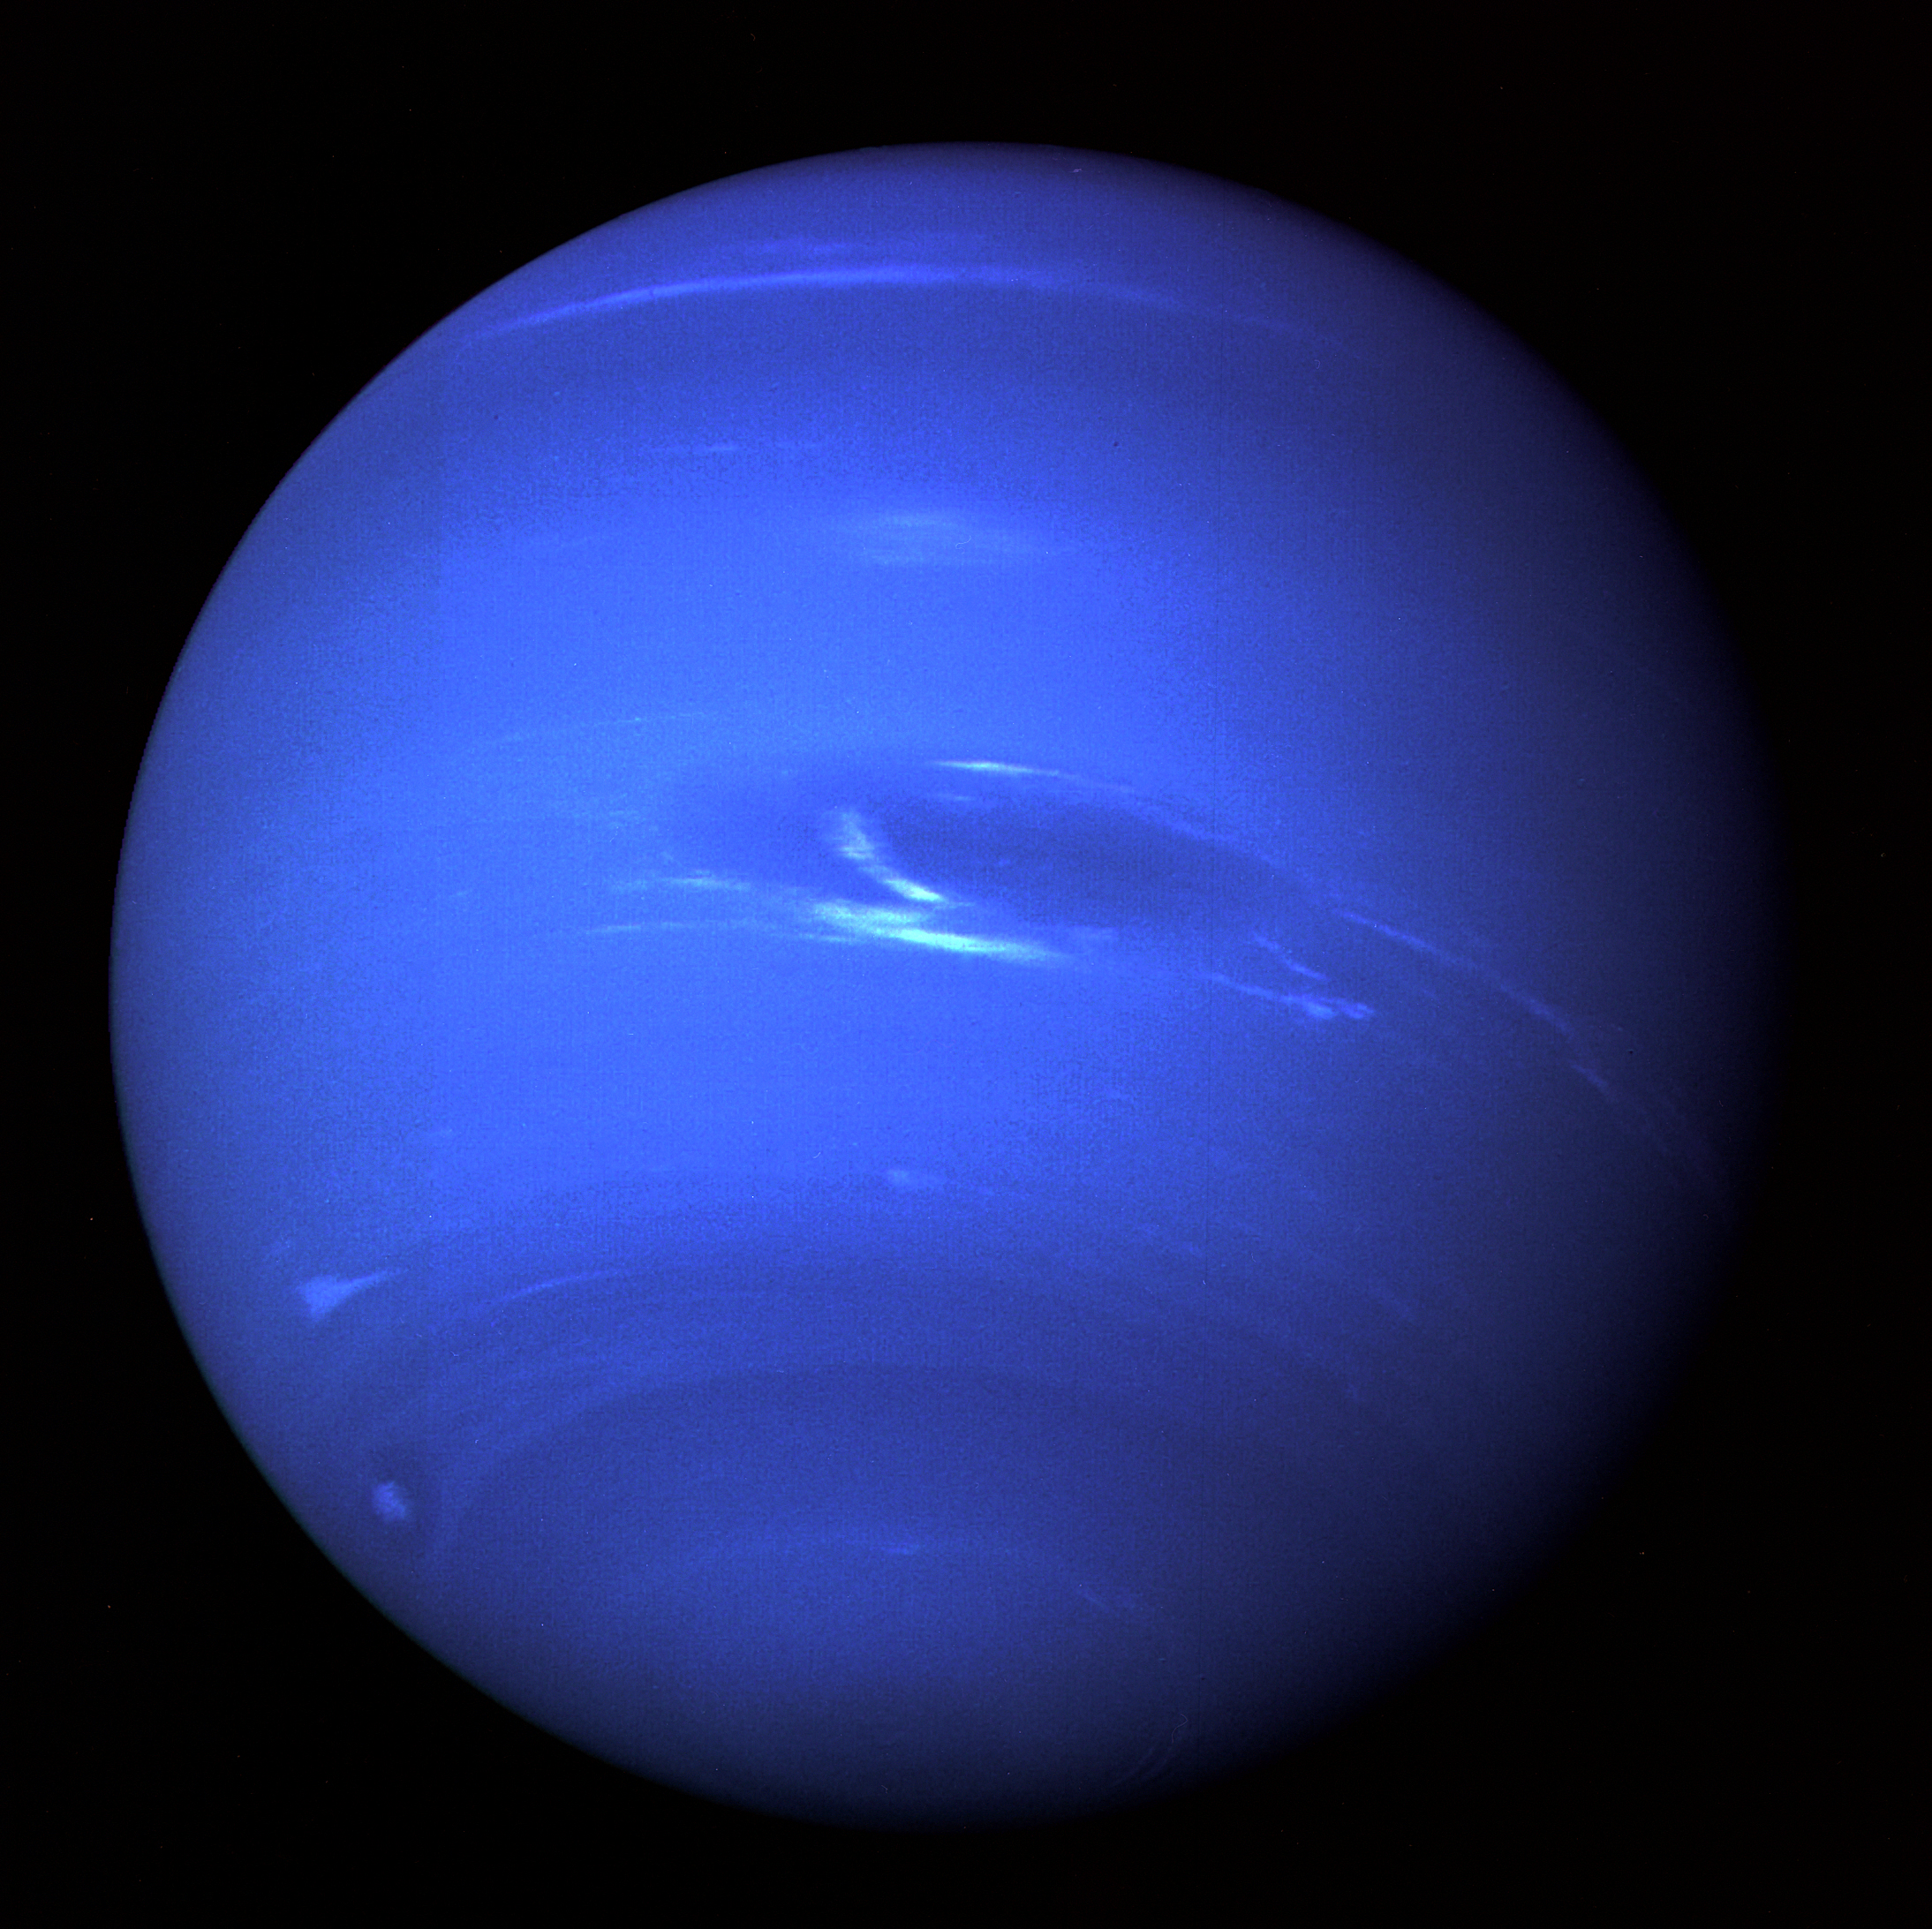
\includegraphics[width=0.5\textwidth]{figures/imageneptune_full.jpg}}~
        \subcaptionbox{Voyager 2 Trajectory\label{fig:voyager2_traj}}{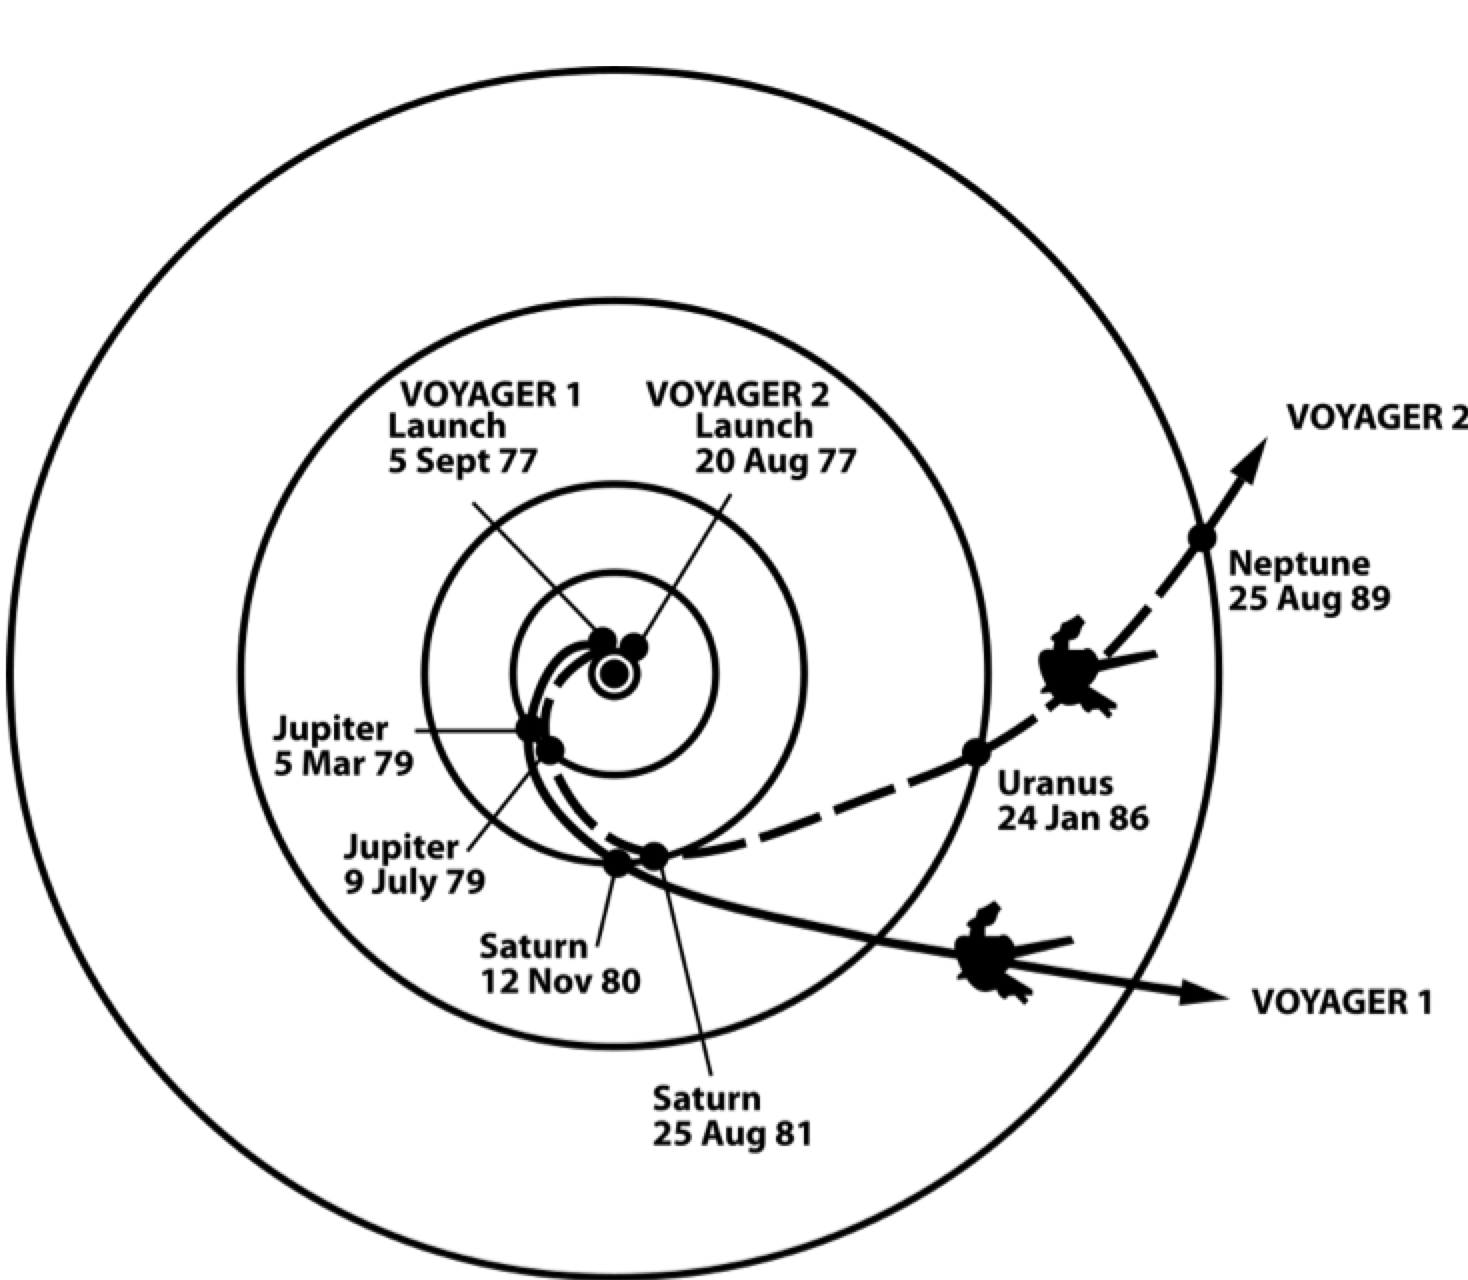
\includegraphics[width=0.5\textwidth]{figures/VoyPlanetTraj.png}}
        \caption{Voyager 2~\label{fig:voyager2}}
    \end{figure}
\end{prob}
\end{document}


